% !TeX root = ../main.tex

\section{Results}
    \subsection{Introduction}
    This study ultimately used the hyperparameters obtained from previous experiments and conducted the final experiments using a GTX 3090. The training process took 3 days, and the following results were obtained.

    \subsection{Result}
    \begin{figure}[htbp]
        \centering
        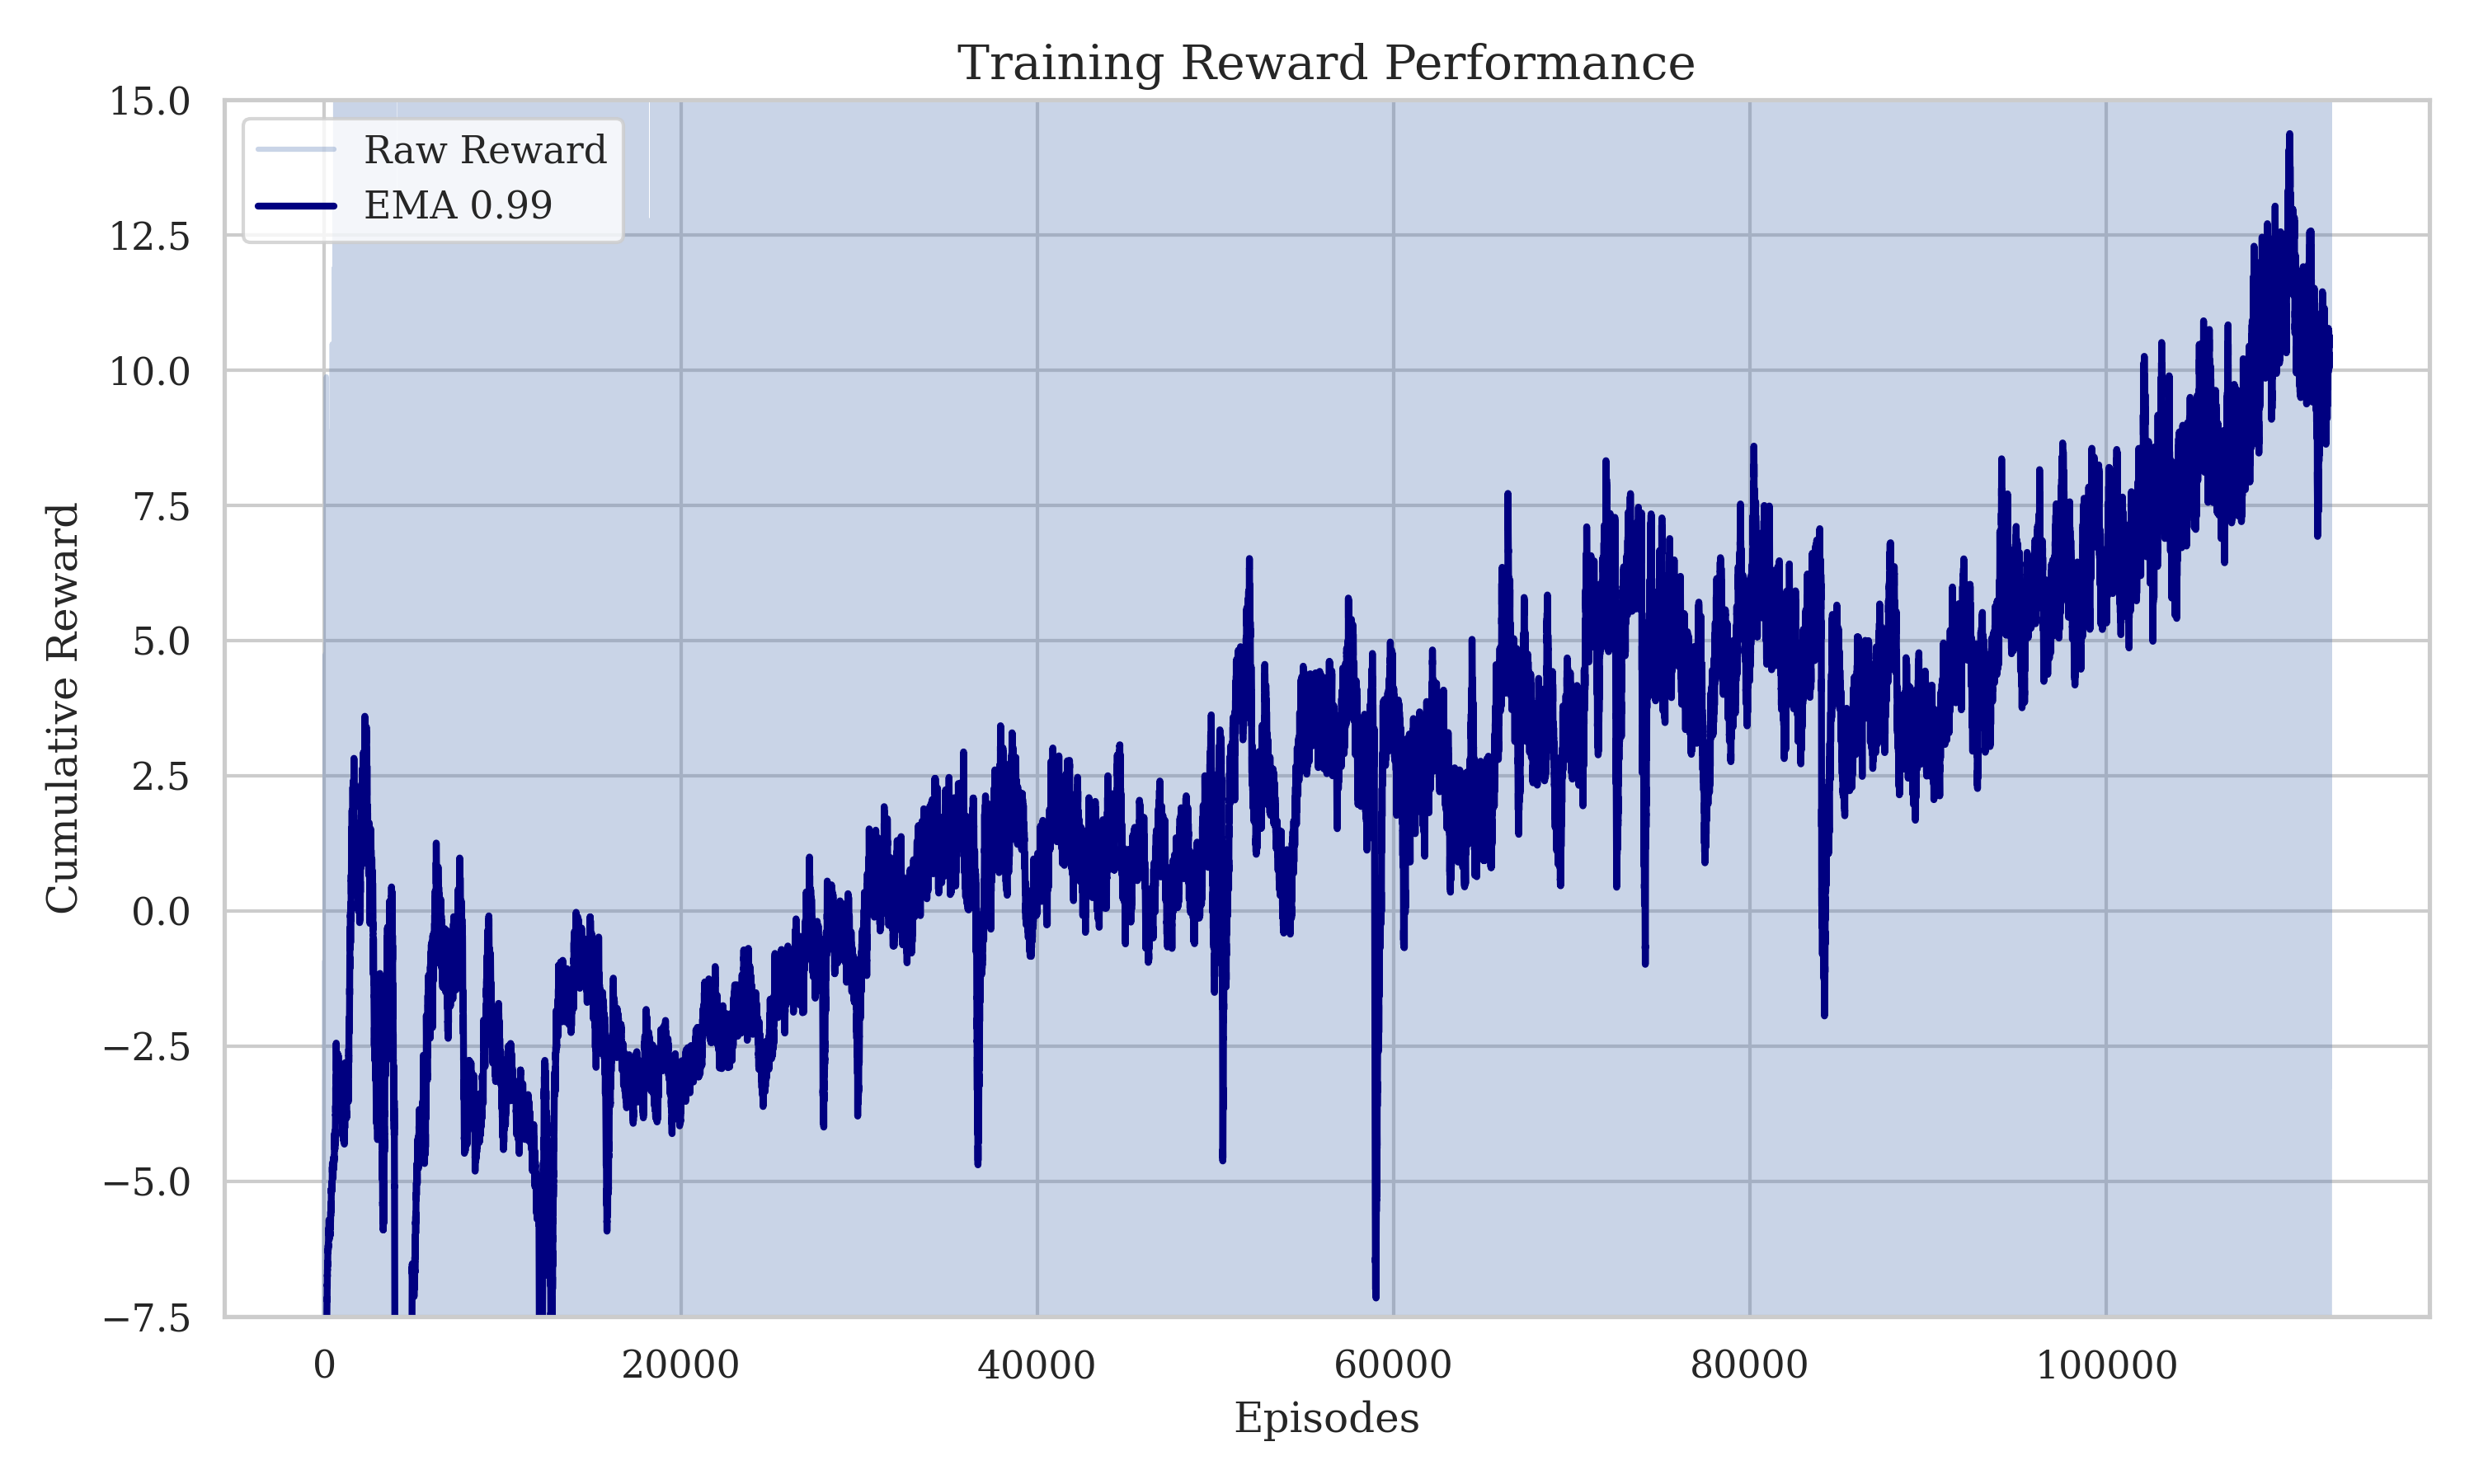
\includegraphics[width=0.3\textwidth]{figures/train reward.png}
        \caption{Train Reward Curve}
        \label{fig:Train Reward Curve}
    \end{figure}

    \begin{figure}[htbp]
        \centering
        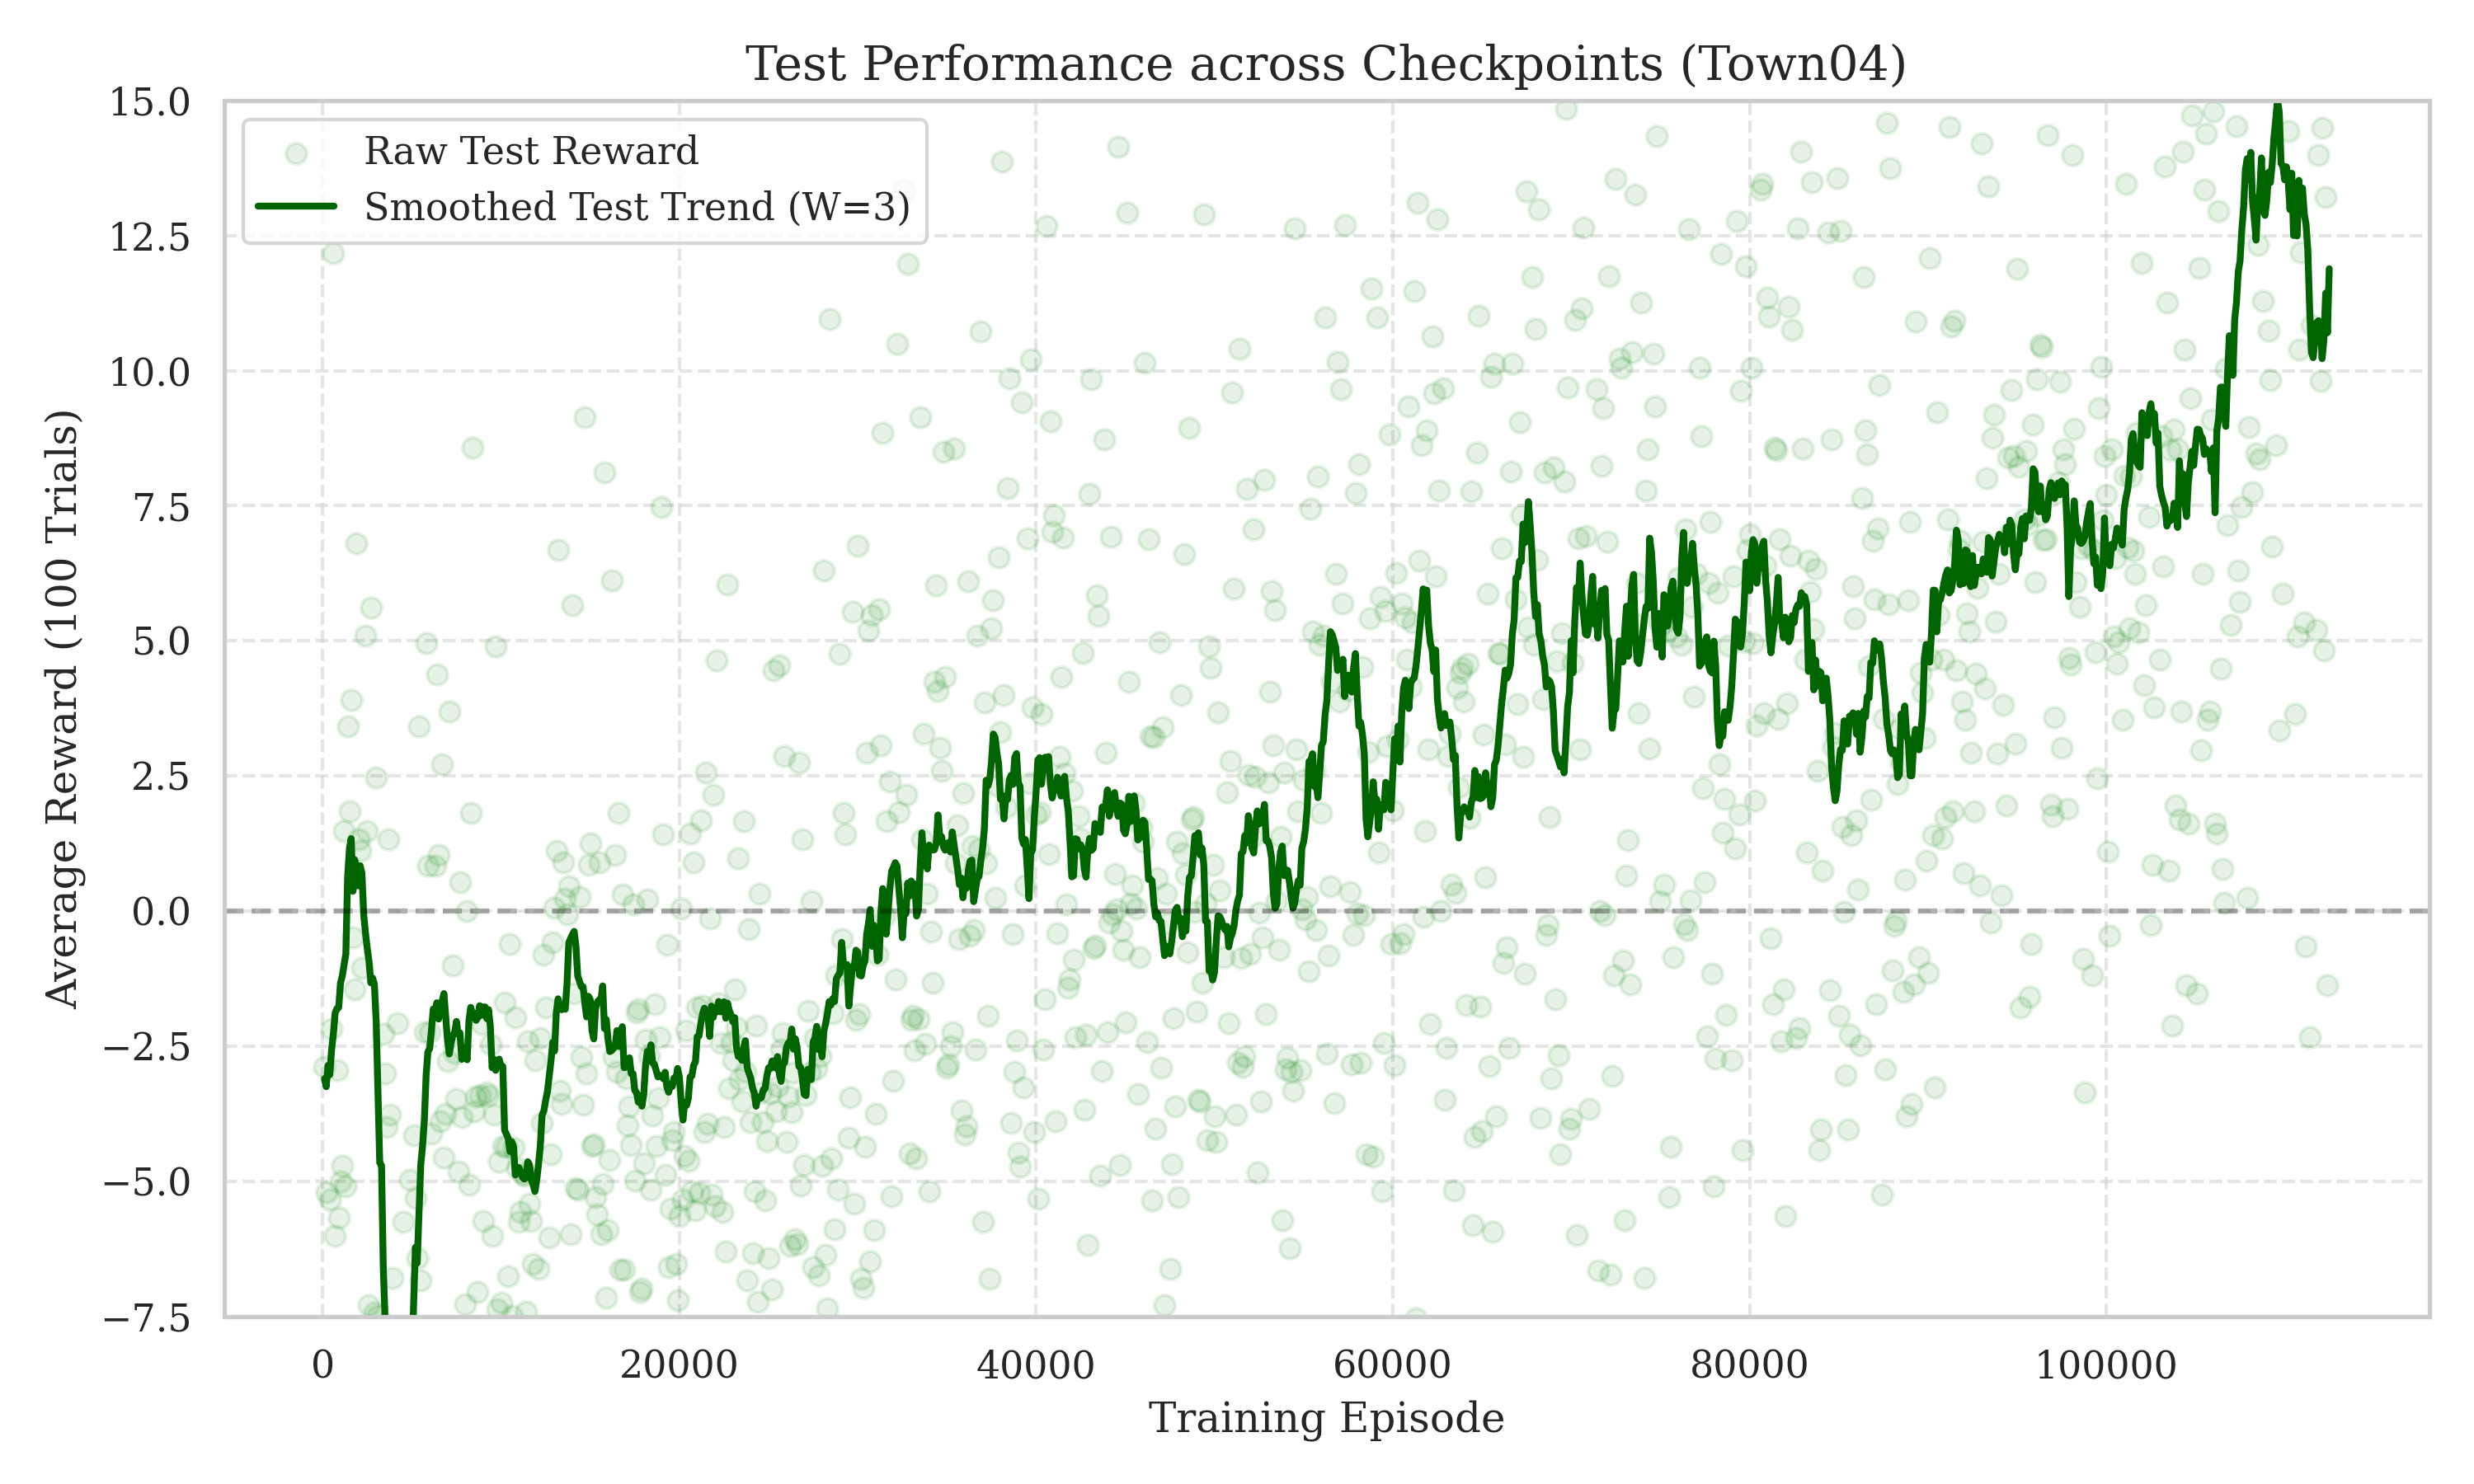
\includegraphics[width=0.3\textwidth]{figures/test reward.png}
        \caption{Test Reward Curve}
        \label{fig:Test Reward Curve}
    \end{figure}

    To evaluate the learning efficiency of ViT-SAC, we recorded the training and evaluation rewards at each checkpoint.

    As shown in \ref{fig:Train Reward Curve} and \ref{fig:Test Reward Curve} , the reward drops significantly in the initial stage of the model. This phenomenon mainly stems from the agent's initial interaction with the simulation environment after completing behavior cloning pre-training, frequently triggering penalties such as collisions and lane incursions when facing unfamiliar states. To avoid collisions or lane incursions, the model adopted a passive strategy to avoid significant penalties. However, due to the introduction of a stopping penalty mechanism, the cumulative penalty of inaction outweighed the risk of exploration. Combined with the inherent maximum entropy mechanism of the SAC algorithm, the agent began to actively explore. Subsequently, the training reward showed a continuous upward trend, rising from a negative baseline to the positive region. Although accompanied by spikes due to high-risk actions, the Double Critic network achieved rapid correction. In the later stages of training, the training reward reached a peak of 15, marking the end of the final training phase of this study.

    The reward curves of the testing and training phases in this study are similar. The environmental parameters are the same for the testing and training phases. The only difference is that the entropy mechanism used for random exploration is turned off in the evaluation phase, and a purely deterministic policy is used for action output.

    \begin{table}[htbp]
    \centering
    \caption{Best Checkpoint Performance Metrics}
    \label{tab:performance_metrics}
    \begin{tabular}{cccc}
    \toprule
    \textbf{Episode} & \textbf{Success Rate} & \textbf{Collision Rate} & \textbf{Offroad Rate} \\ \midrule
    108299 & 58 & 28 & 14\\
    110999 & 50 & 34 & 16\\
    109399 & 48 & 36 & 16\\
    108699 & 44 & 48 & 8\\
    107699 & 42 & 44 & 14\\
    \bottomrule
    \end{tabular}
    \end{table}

    These are the final results of this study. The testing method involved conducting five random intersection tests on each checkpoint. Then, the 25 best-performing checkpoints were selected for more detailed testing. In the detailed testing phase, 50 intersections were randomly selected to obtain a more realistic assessment of the checkpoints' capabilities. The above are the five best-performing checkpoints in this study. The best-performing checkpoint was 108299, with a success rate of 58\%, a collision rate of 28\%, and a road exit rate of 14\%.